\documentclass[../main.tex]{subfiles}

\begin{document}
    \section{Сравнение с экспериментом}
    В ходе большого числа экспериментов по описанной выше методике было установлено, что пороговая энергия 
    Оже-рекомбинации структуры рассчитаная в изотропном приближении неплохо кореллирует с температурой затухания 
    вынужденного излучения в образце . При этом существует примерное равенство \cite{TmaxEthEq}:
    \begin{equation}
        T_{max} \approx E_{th} / 2;
    \end{equation}

    Это может быть объяснено, если учесть крайне высокие темпы термолизации носителей, что приводит
    к распределению, близкому к Больцмановскому.

    Рассмотрим для начала образец, предназначенный для излучения на длине волны $14~nm$.

    Результаты расчётов спектра электронов и дырок для двух случаев приведены на рисунке. В первом случае (рис. а) расчёт
    проведён для экспериментально исследованной Cd0.1Hg0.9Te/Cd0.65Hg0.35Te КЯ толщиной 7.4 нм, во втором случае (рис. б)
    расчёт проведён для HgTe/Cd0.65Hg0.35Te КЯ толщиной 4.3 nm. В обоих случаях ширина запрещённой зоны составляет при 
    80 K порядка $83~meV$. 

    \begin{figure}[h]
        \begin{minipage}[h]{0.45\linewidth}
            \begin{center}
                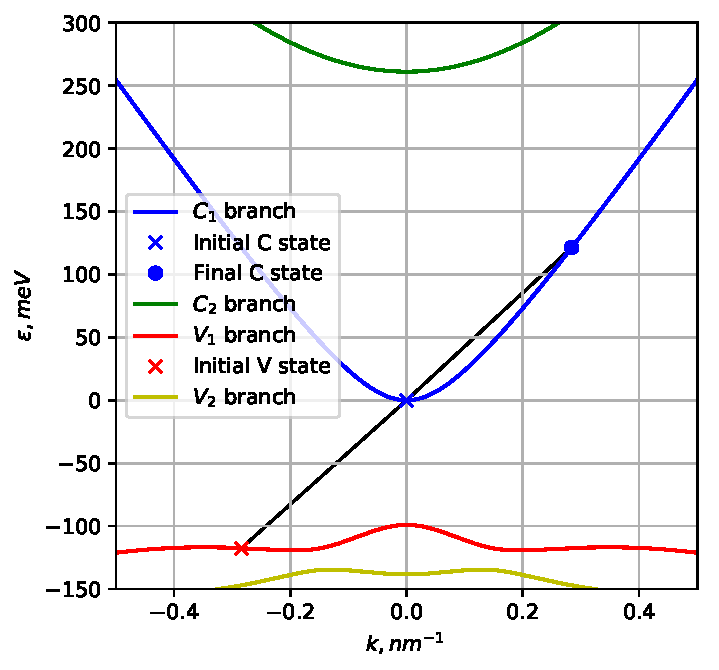
\includegraphics[width=1.\linewidth]{./images/main_14u_80K_pic.pdf}

                \textbf{Рис. а: Образец с "грязными" КЯ.} Пороговая энергия 
                    $\varepsilon_{th} \approx 18.4~meV$.
            \end{center}
        \end{minipage}
        \hfill
        \begin{minipage}[h]{0.45\linewidth}
            \begin{center}
                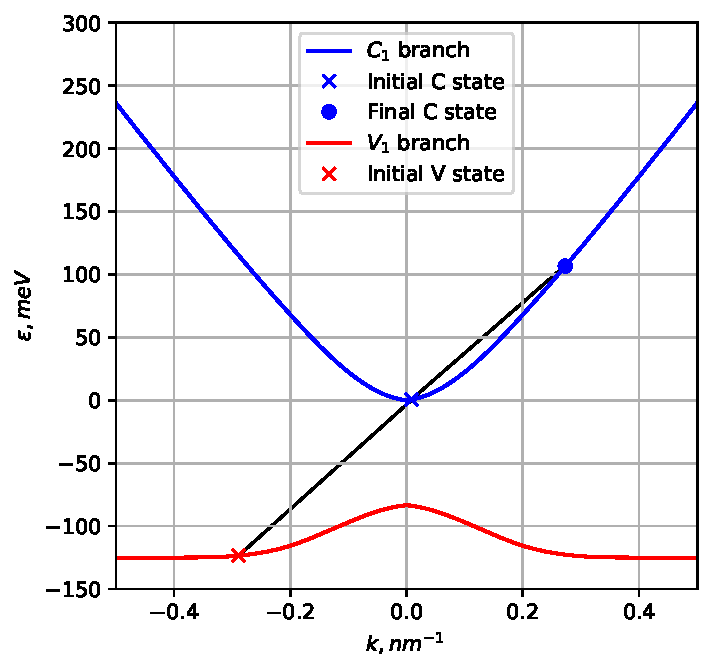
\includegraphics[width=1.\linewidth]{./images/14u_pure_80K.pdf}

                \textbf{Рис. б: Образец с "чистыми" КЯ.} Пороговая энергия 
                    $\varepsilon_{th} \approx 23.3~meV$.
            \end{center}
        \end{minipage}
    \end{figure}

    Как правило достаточно рассмотреть CCHC процесс, где электроны находятся на нижней подзоне, а "дырки" соответственно на верхней,
    поскольку в большинстве структур именно он имеет наименьшую пороговую энергию, однако иногда это не справедливо.

    %\begin{center}
    %    \begin{tabular}{c | c | c | c | c}
    %        Состав ямы, x & Состав барьера, x & Ширина ямы, nm& $E_g$    & $E_{th}$\\
    %        \hline
    %        0.097 & 0.65    &  7.4 & 82.4    & 15.8\\
    %        \hline
    %        0.1 & 0.65      & 7.4  & 86 & 12.8\\
    %        0.0 & 0.65      & 3.9   & 82.4  & 20.3\\
    %        0.097   & 0.67  & 7.4  & 81gi.4  & 25.9\\
    %    \end{tabular}
    %\end{center}


    Также рассмотрим струтуру, расчитанную на $18\mu m$. 
    Результаты расчётов спектра электронов и дырок для двух случаев приведены на рис. 1. В первом случае (рис. 1 а) расчёт проведён 
    для экспериментально исследованной Cd0.1Hg0.9Te/Cd0.65Hg0.35Te КЯ толщиной 8.7 нм, во втором случае (рис. 1 б) расчёт проведён для 
    HgTe/Cd0.65Hg0.35Te КЯ толщиной 4.4 nm.

    \begin{figure}[h]
        \begin{minipage}[h]{0.45\linewidth}
            \begin{center}
                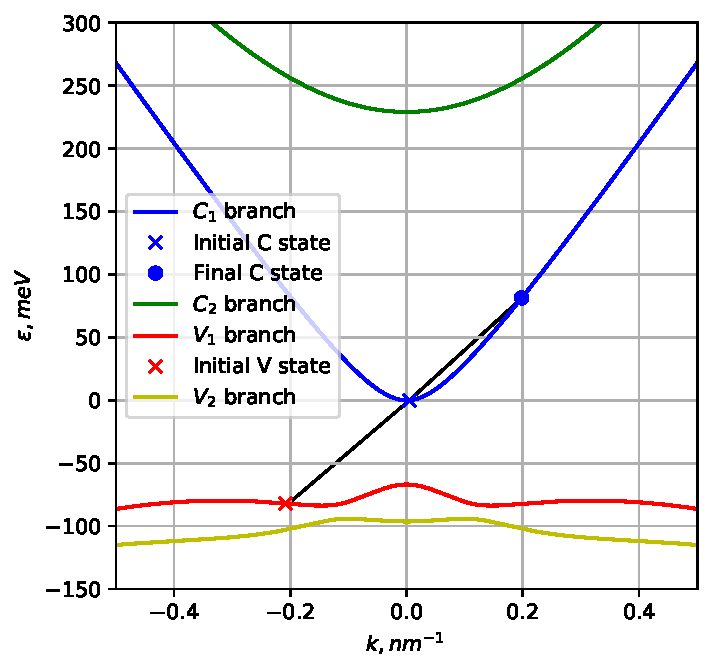
\includegraphics[width=1.\linewidth]{./images/18u_impure_40K.pdf}

                \textbf{Рис. а: Образец с "грязными" КЯ.} Пороговая энергия 
                    $\varepsilon_{th} \approx 15~meV$.
            \end{center}
        \end{minipage}
        \hfill
        \begin{minipage}[h]{0.45\linewidth}
            \begin{center}
                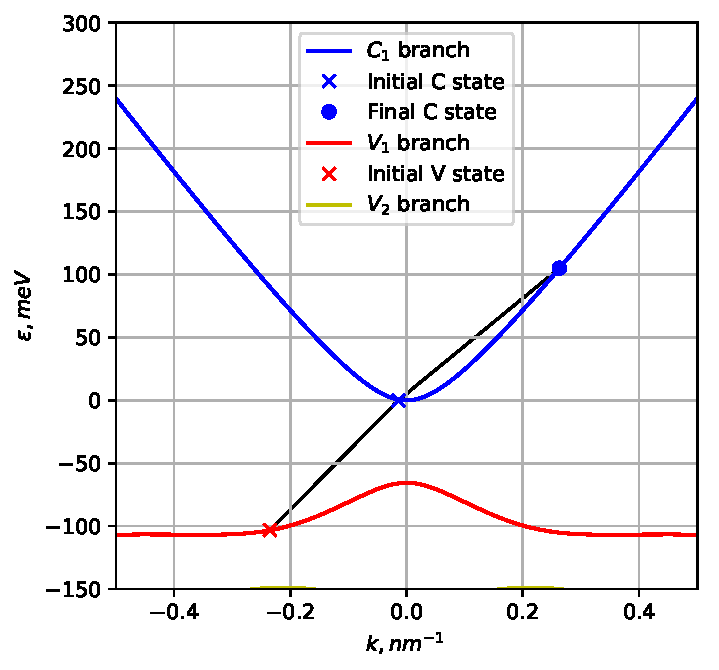
\includegraphics[width=1.\linewidth]{./images/18u_pure_40K.pdf}

                \textbf{Рис. б: Образец с "чистыми" КЯ.} Пороговая энергия 
                    $\varepsilon_{th} \approx 37.3~meV$.
            \end{center}
        \end{minipage}
    \end{figure}

    Из рисунка a видно, что для первого случая в валентных подзонах имеются дополнительные максимумы, располагающиеся ниже потолка валентной 
    зоны на 7 мэВ. В HgTe яме, окруженной Cd0.65Hg0.35Te, эти экстремумы практически отсутствуют (рис. б). Как будет показано ниже, вид 
    закона дисперсии дырок будет важен при определении величины пороговой энергии оже-рекомбинации.

    Интересно сравнить пороговые энергии для структуры, описанной выше, и структур на основе квантовых ям HgTe. На рисунке ниже представлена 
    зависимость пороговой энергии оже-рекомбинации (вычисленной в модели) и толщины КЯ при двух разных концентрациях состава ям
    от доли Cd в барьерах для температуры 40K, 
    при фиксированной величине ширины запрещённой зоны, составляющей $67~meV$. Из рисунка видно, что максимальная пороговая энергия (что оптимально 
    с точки зрения максимальной температуры генерации стимулированного излучения) достигает величины 38 meV при доле Cd 0.67 и чистой яме, а также 
    17 meV при высоте барьеров в 0.5.
    \vspace{0.75cm}
    \begin{minipage}[h]{\linewidth}
        \begin{center}
            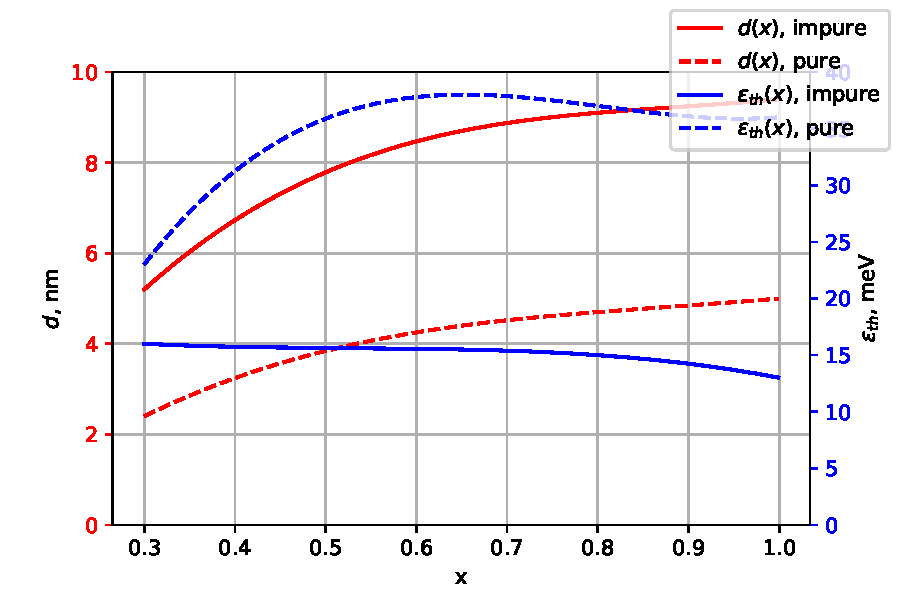
\includegraphics[width=1.\linewidth]{./images/de_vs_x.pdf}

            \vspace{0.75cm}
            \textbf{Пороговая энергия Оже-процесслв и толщина КЯ.}
            Расчеты проводились при $T= 40K$, $E_g \approx 67~meV$.
            \vspace{1.25cm}
        \end{center}
    \end{minipage}

    Для объяснения различия пороговых энергий в квантовых ямах HgTe и Cd0.1Hg0.9Te на !!! приведены начальные и конечные состояния электронов 
    и дырок, соответствующие порогу оже-рекомбинации. Из сравнения видно, что «эффективная масса» дырок для оже-процесса в HgTe квантовой яме 
    существенно меньше, чем в Cd0.1Hg0.9Te квантовой яме. Это связано с наличием в в Cd0.1Hg0.9Te квантовой яме ярко выраженного бокового 
    экстремума в верхней валентной подзоне. Хорошо известно, что увеличение эффективной массы дырок приводит к снижению пороговой энергии 
    Оже-процесса. Наличие максимума на зависимости пороговой энергии от доли кадмия в HgTe/CdxHg1-xTe обусловлено наличием минимума 
    «эффективной массы» дырок при определенной доле кадмия. Следует отметить, условность использованного здесь термина «эффективная масса» 
    для верхней валентной подзоны, поскольку закон дисперсии в ней не квадратичный и, вообще говоря, немонотонный.

    Таким образом, было продемонстрировано, что при заданной энергии межзонного перехода пороговая энергия оже-рекомбинации в структурах 
    HgTe/CdxHg1-xTe с КЯ является немонотонной функцией от доли кадмия в барьере. При оптимальной концентрации кадмия в барьерах и КЯ из HgTe 
    можно ожидать почти трехкратного повышения критической температуры стимулированного излучения по сравнению с прототипной структурой с 
    Cd0.1Hg0.9Te/Cd0.65Hg0.35Te КЯ.
\end{document}